
% This is samplepaper.tex, a sample chapter demonstrating the
% LLNCS macro package for Springer Computer Science proceedings;
% Version 2.20 of 2017/10/04
%
\documentclass{llncs}
\usepackage{graphicx}
\makeatletter
\@twosidefalse
\@mparswitchfalse
\makeatother
\usepackage{amsmath}
\usepackage{hyperref}
\usepackage{setspace}
\onehalfspacing
\usepackage{float}
\pagestyle{headings}
\setcounter{tocdepth}{8}
\hypersetup{%
    pdfborder = {0 0 0}
}
\renewenvironment{abstract}{
  \begin{center}%
    {\large\bfseries Abstract}
  \end{center}
  \quotation
}
{
  \endquotation
}
\usepackage{sectsty}
\sectionfont{\fontsize{15}{14}\selectfont}
\subsectionfont{\fontsize{13}{13}\selectfont}

\usepackage{graphicx}
% Used for displaying a sample figure. If possible, figure files should
% be included in EPS format.
%
% If you use the hyperref package, please uncomment the following line
% to display URLs in blue roman font according to Springer's eBook style:
% \renewcommand\UrlFont{\color{blue}\rmfamily}
\begin{document}
%

\title{

\begin{figure}[ht]
    \centering
    
\includegraphics[width=1\linewidth]{concordia.jpeg}
    \label{fig:example}
\end{figure}

What should I consider when setting
up software tools I will be using to
coordinate many interrelated projects?\vspace{5pt}}
%
%\titlerunning{Abbreviated paper title}
% If the paper title is too long for the running head, you can set
% an abbreviated paper title here
%
\author{\large \textbf{Khyati Bareja - Student ID: 40221300}\vspace{20pt}}
%
%
\institute{\large \textbf{SOEN 6841- Software Project Management} \\
\vspace{15pt} \textbf{Advisor: Pankaj Kamthan} \\
\vspace{60pt} \textbf{Computer Science and Software Engineering , Concordia University} \\
\vspace{15pt} \textbf{ VCS: Github: \href{https://github.com/Khyati-Bareja/SOEN6481-TAS}{https://github.com/Khyati-Bareja/SOEN6481-TAS}}}

{\def\addcontentsline#1#2#3{}\maketitle}
\newpage

\section{Abstract}
The approaches and crucial factors that must be taken into account when creating software tools to manage several connected projects are highlighted in this study. The emphasis is on how important it is to comply with industry norms, organizational requirements, regulatory frameworks, and program management office suggestions, and also using a strong Project or Program Management Information System, to exercise control and make work collaboration easier. The adoption of software packages with sophisticated capabilities is highlighted, as is the strategic way of organizing online data for easy accessibility by remote project teams. Additionally, in order to improve organizational clarity, the study supports, careful recording of the staffing hierarchy inside the program and assigning tasks to a designated program owner. It is advised that centralized, sophisticated technologies be used to support general uniformity. One of the most important practices for attaining complete and unified project management is having program staff participate in project starting workshops and planning meetings.



\tableofcontents
\newpage

\section{Introduction}

\subsection{Motivation}
The corporate landscape of today is multifaceted. Managers must be able to act quickly, distribute limited resources effectively, and maintain focus. Management faces a variety of difficulties with businesses that are working on several projects at once which are interrelated. Particular issues arise for project managers in charge of several projects with various scopes, levels of complexity, and deadlines. These may have to do with throughput times and conflicts over resources. When limited resources are not properly balanced, the organization is frequently under more strain, which results in poor information quality and longer project lead times.~\cite{refpaper1}

Hence, setting up an effective project or program management information system(PMIS) and utilizing software tools to coordinate interrelated projects becomes necessary for maintaining coordination and control over ongoing activities and to organize online information so that members of remote project teams may quickly locate the information they require. This may in turn help the management to coordinate their distributed and interrelated projects and contribute in better decision making, by avoiding resource overlapping,provisioning the easy delegation of work, evaluation and estimation of costs and plan changes accordingly and in parallel.~\cite{refpaper1}

\subsection{Problem Statement}
The problem statement addressed here is about the factors to consider when setting up software tools to coordinate multiple interrelated projects. This includes:
\begin{enumerate}
  \item Assessing all the information requirements that the program will need to comply with, determining how to meet them, and establishing an effective project or program management information system (PMIS) to control and coordinate ongoing work and coordinating program plans.

 \item Monitoring Progress via use of common computer scheduling tools for all projects within the program.

\end{enumerate}


\subsection{Objectives}
Objectives Depends on majorly three factors,
\begin{enumerate}
\item \textbf{Organizational requirements}:
\subitem Evaluate program information requirements for compliance with rules and guidelines and establish or leverage infrastructure for storing project data, considering long-term obligations.
\item \textbf{Program management office (PMO) recommendations}: \subitem Setting up up an effective Program Management Information System (PMIS) for control and coordination.
\subitem Explore advanced options to enhance information infrastructure capabilities.
\item \textbf{Regulations and industry standards and Access}:
\subitem Clearly documenting staffing hierarchy, roles, responsibilities, and contact information to better coordinate among inter-related projects, as per industry standards.
\subitem Ensuring access to common scheduling tools for all projects.
\subitem Adopt compatible project management software, providing training and expertise to coordinate program plans.
\subitem Standardizing processes for status collection and reporting, ensuring consistency throughout the programs.

\end{enumerate}

\section{Background Material}
The topic of Inter-related Projects and mitigating its impact on the project by managing it in better ways collectively has been in research from some time now. On the basis of proven studies there are various categorization of these interdependencies and how they affect the project management. \\
\textbf{Types of Interdependencies between Multiple Projects:}
\begin{enumerate}
\item \textbf{External Interdependencies:} These are influenced by factors external to the organization, such as social and economic changes. For example, a sudden change in market conditions can lead to priority variations in the projects within a portfolio or outside.~\cite{refpaper2}
\item \textbf{Internal Interdependencies:} These arise when the resource requirements or benefits of one project are significantly affected by the selection or rejection decisions of other projects within the set. For instance, an unexpected delay in one project can impact other dependent projects, leading to an overall delay in the completion time of a new product or service.~\cite{refpaper2}
\item \textbf{Resource Interdependencies:} These occur when there is a need to share resources or wait for scarce resources until another project releases them. Improper management of resource interdependencies can result in resource waste.~\cite{refpaper2}
\item\textbf{Technology Interdependencies:} These involve leveraging common technology across multiple projects. If not properly managed, technology interdependencies can lead to schedule slippage.~\cite{refpaper2}
\item \textbf{Technical Interdependencies:} These arise from the need to address technical challenges that cut across multiple projects. Ineffective management of technical interdependencies can result in budget waste. \item\textbf{Learning-based Interdependencies:} These stem from the need to incorporate the capabilities and knowledge gained from previous projects. Poor management of learning-based interdependencies can hinder knowledge diffusion and innovation.~\cite{refpaper2}
\end{enumerate}
Along with the above mentioned there exist other landscape of interdependencies among project activities and tasks as well,that can further be categorized on varying level of interdependence as  'flow,' 'fit,' and 'sharing.'~\cite{refpaper5} \\
\textbf{Problems Caused by Poor Project Interdependencies Management can be:}
\begin{enumerate}
\item \textbf{Wastage of Resources:} Inadequate consideration of project interdependencies can result in inefficient resource utilization, leading to resource waste.~\cite{refpaper2}~\cite{refpaper3}
\item \textbf{Schedule Slippage:} When interdependent projects are not properly managed, a delay in one project can propagate to other interconnected projects, causing overall schedule slippage.~\cite{refpaper2}~\cite{refpaper3}
\item \textbf{Budget Wastage:} Failure to consider interdependencies among projects during the selection process can lead to unnecessary duplication of efforts and resources, resulting in budget waste.~\cite{refpaper2}
\item\textbf{Inter-project Competition:} When projects start competing for scarce resources, it can lead to conflicts and hinder the achievement of project objectives.~\cite{refpaper2}~\cite{refpaper4}
\item\textbf{Impact on Cost:} The cost of managing project interdependencies can be impacted in various ways. Poor management of interdependencies can lead to resource waste, schedule slippage, and budget waste, all of which can increase project costs. On the other hand, effective management of interdependencies can optimize resource utilization, prevent delays, and reduce unnecessary expenses, resulting in cost savings.~\cite{refpaper2}
\end{enumerate}
Hence, enhancing project management by equipping project managers with sophisticated analytical tools, will envision to help manage the complexity of interdependent projects by offering insights into information flow and critical activities for more informed decision-making and optimized project outcomes.~\cite{refpaper5}


\section{Methods \& Methodology}
%Managing knowledge
The Methodologies that should be adapted when setting up software tools for interrelated/interdependent Projects:
\begin{enumerate}
      \item \textbf{Centralized Project Management :}
      \subitem Consider centralized, high-end project management tools for advantages in coordination. Provide training to all users and establish expertise within the program team. Budget for costs and efforts required and assess processes for synchronizing plans and schedules.\\
      Example : \textbf{Kanban} can be beneficial in managing interrelated projects, especially when those projects share resources, dependencies, or have interconnected workflows.
        \begin{figure}
            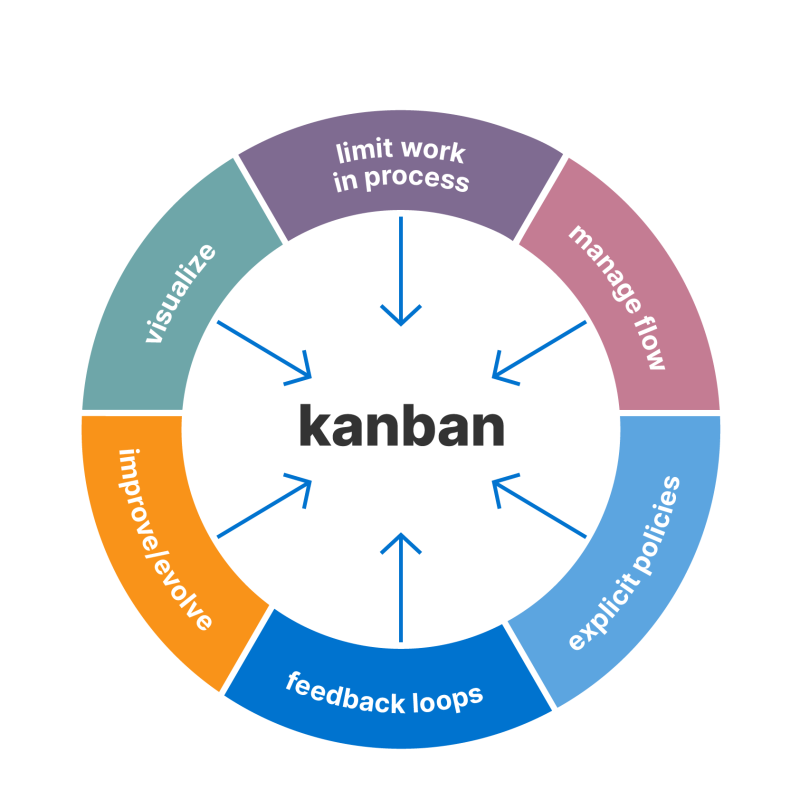
\includegraphics[width=0.3\linewidth]{Kanban_map.png}
            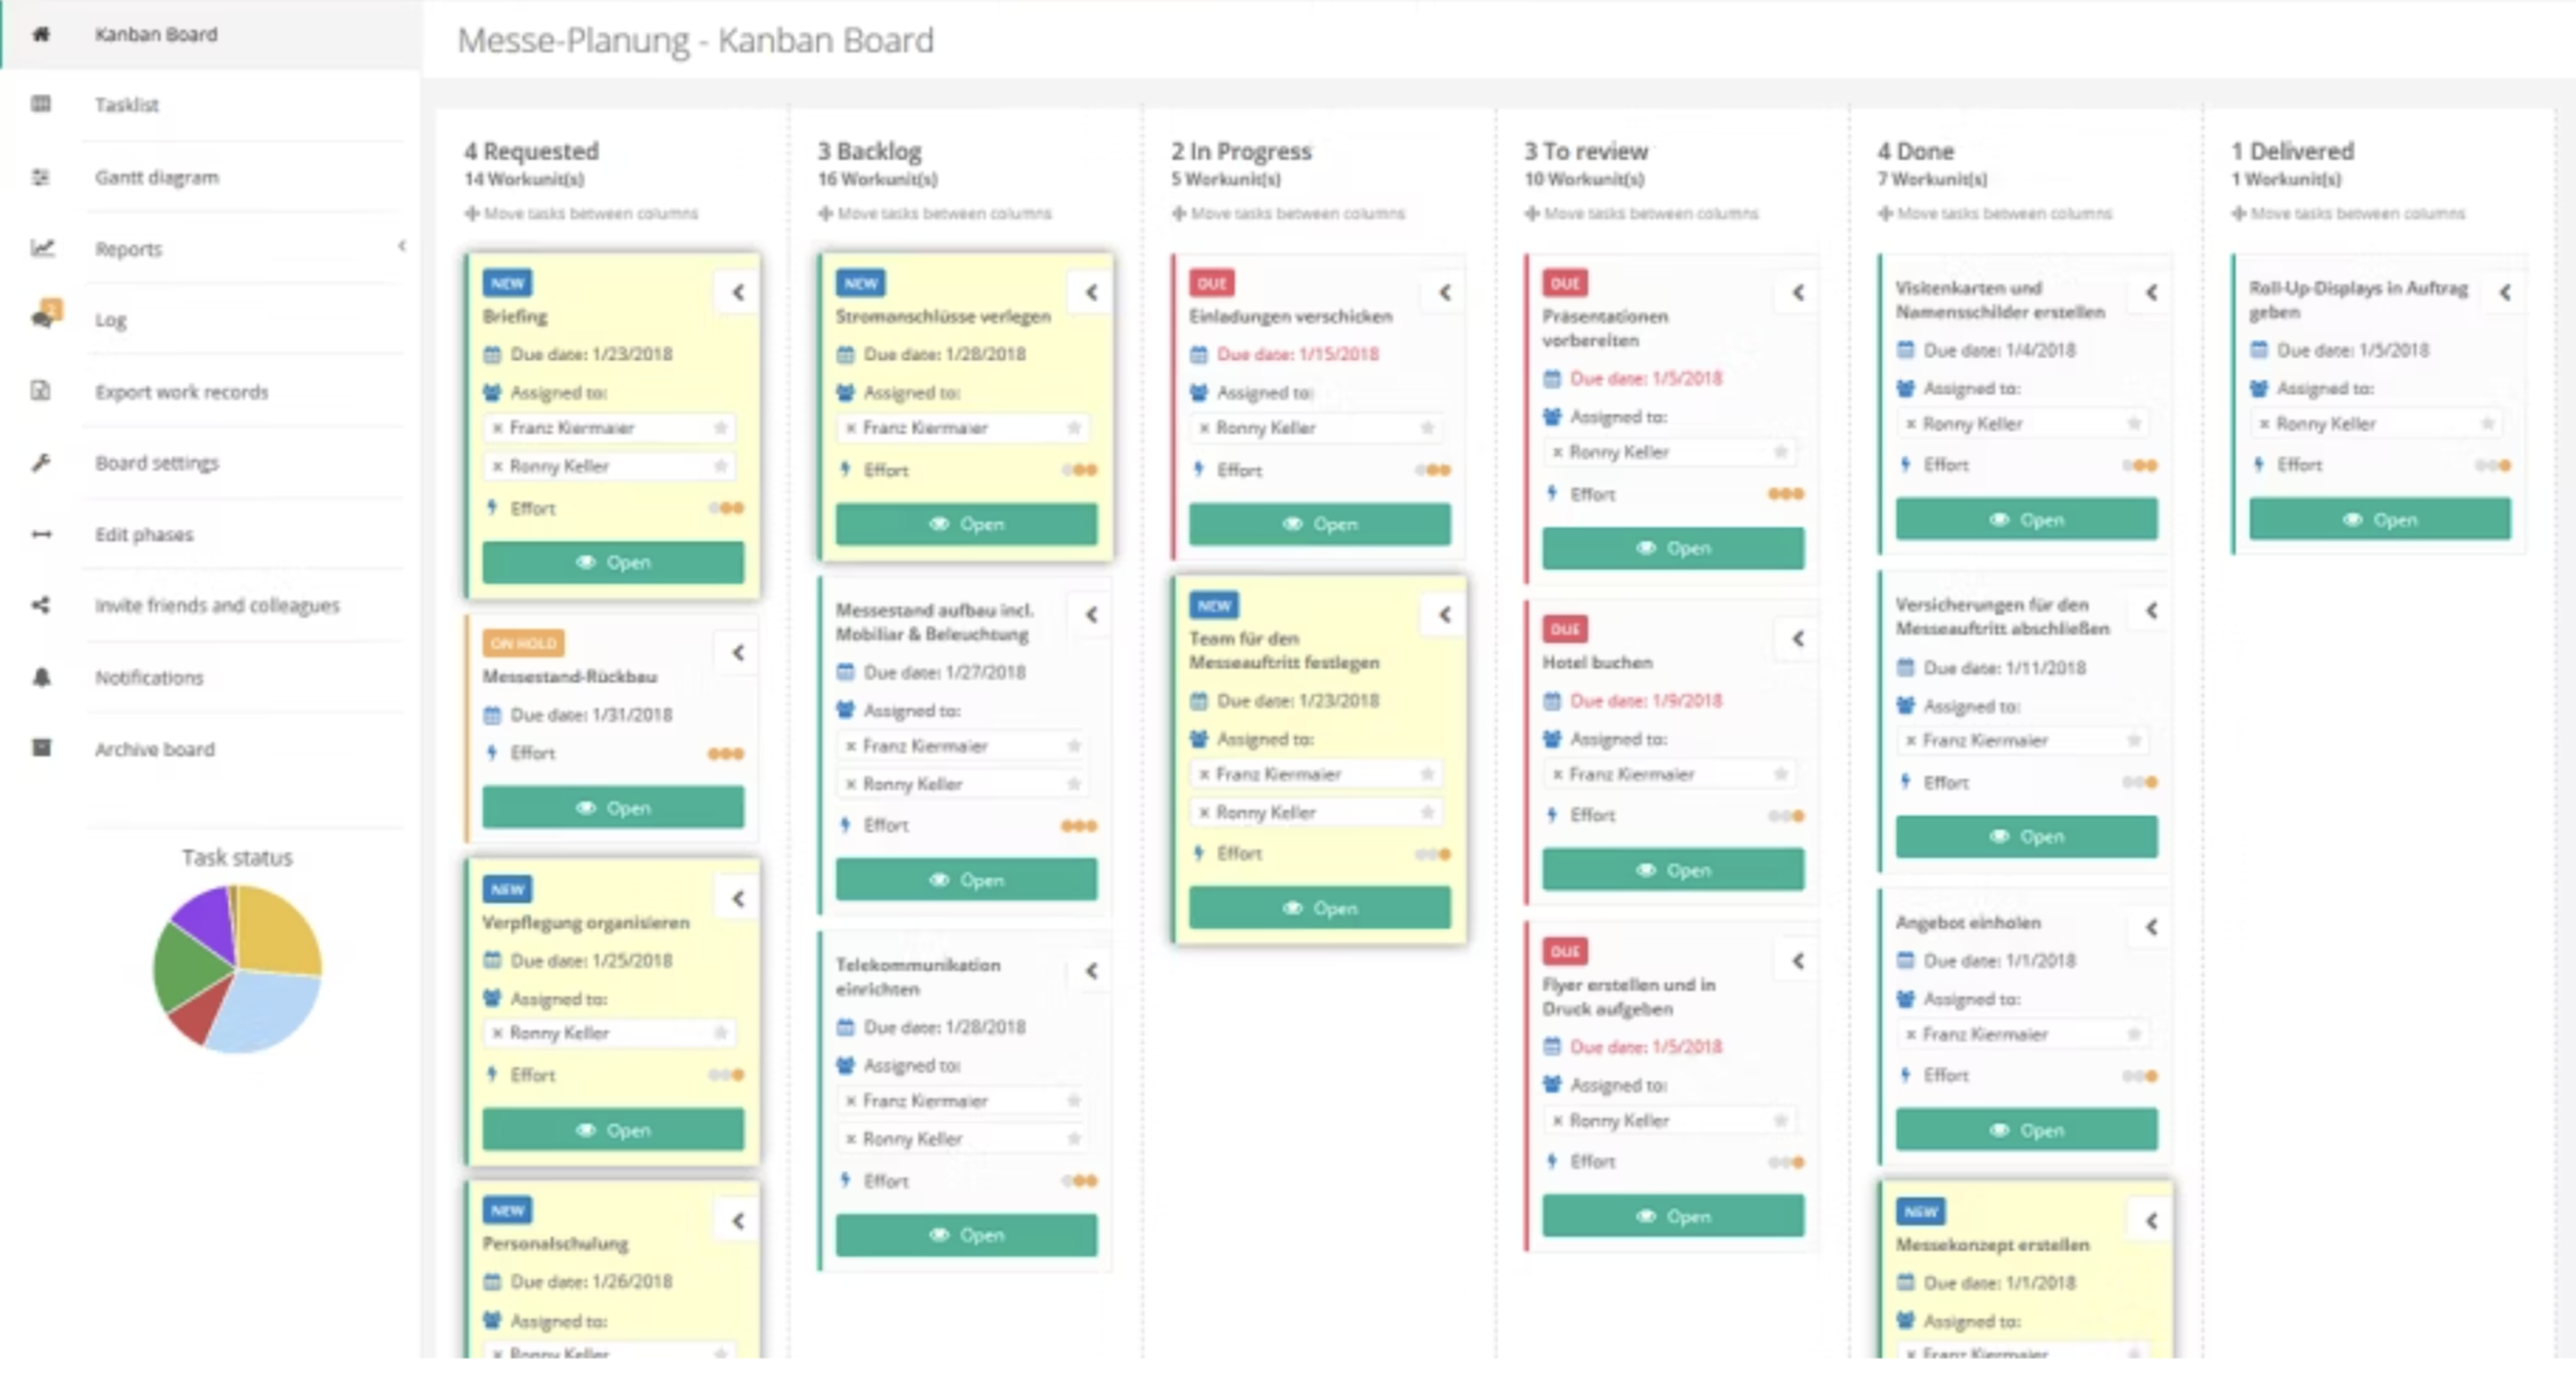
\includegraphics[width=0.75\linewidth]{KanbanBoard.png}

        \end{figure}
        \begin{enumerate}
            \item Kanban employs a visual board to represent the workflow: When managing interrelated projects, you can use a Kanban board to visualize the tasks and activities related to each project.~\cite{refpaper6} This allows teams to have a clear understanding of the work in progress, bottlenecks, and dependencies.~\cite{refpaper6}
            \item Transparency Across Projects: With a Kanban board, teams can easily see the status of tasks and projects in real-time. This transparency is crucial when managing interrelated projects, as it helps in identifying potential conflicts, resource constraints, or delays.~\cite{refpaper6}
            \item Work Prioritization: Kanban allows for the clear prioritization of work items. When managing multiple projects, teams can use Kanban to prioritize tasks based on the overall goals and objectives of the organization. This helps in ensuring that the most critical and high-priority tasks are addressed first.~\cite{refpaper6}
            \item Managing Dependencies: Kanban can help in managing dependencies between tasks and projects. By visualizing and tracking dependencies on the Kanban board, teams can identify potential blockers early and take necessary actions to mitigate risks.~\cite{refpaper6}
        \end{enumerate}
    \item\textbf{Critical Chain Project Management (CCPM):}
    This an approach focuses primarily on the management of the duration of activities, considering the allocation of resources, that originated from the Theory of Constraints (TOC) and is designed to improve the efficiency and effectiveness of project management. While CCPM is commonly associated with single-project environments, it can also be adapted for managing multiple interrelated projects within a larger program. \\
    \textbf{Case Study:}To conduct a comprehensive analysis and understand the behavior of the CCPM method in a real multiproject environment, a case study was performed in a tooling manufacturing company for the construction industry facing a complex environment with projects competing for the use of resources.~\cite{refpaper7}
                \begin{figure}
                    \centering
                    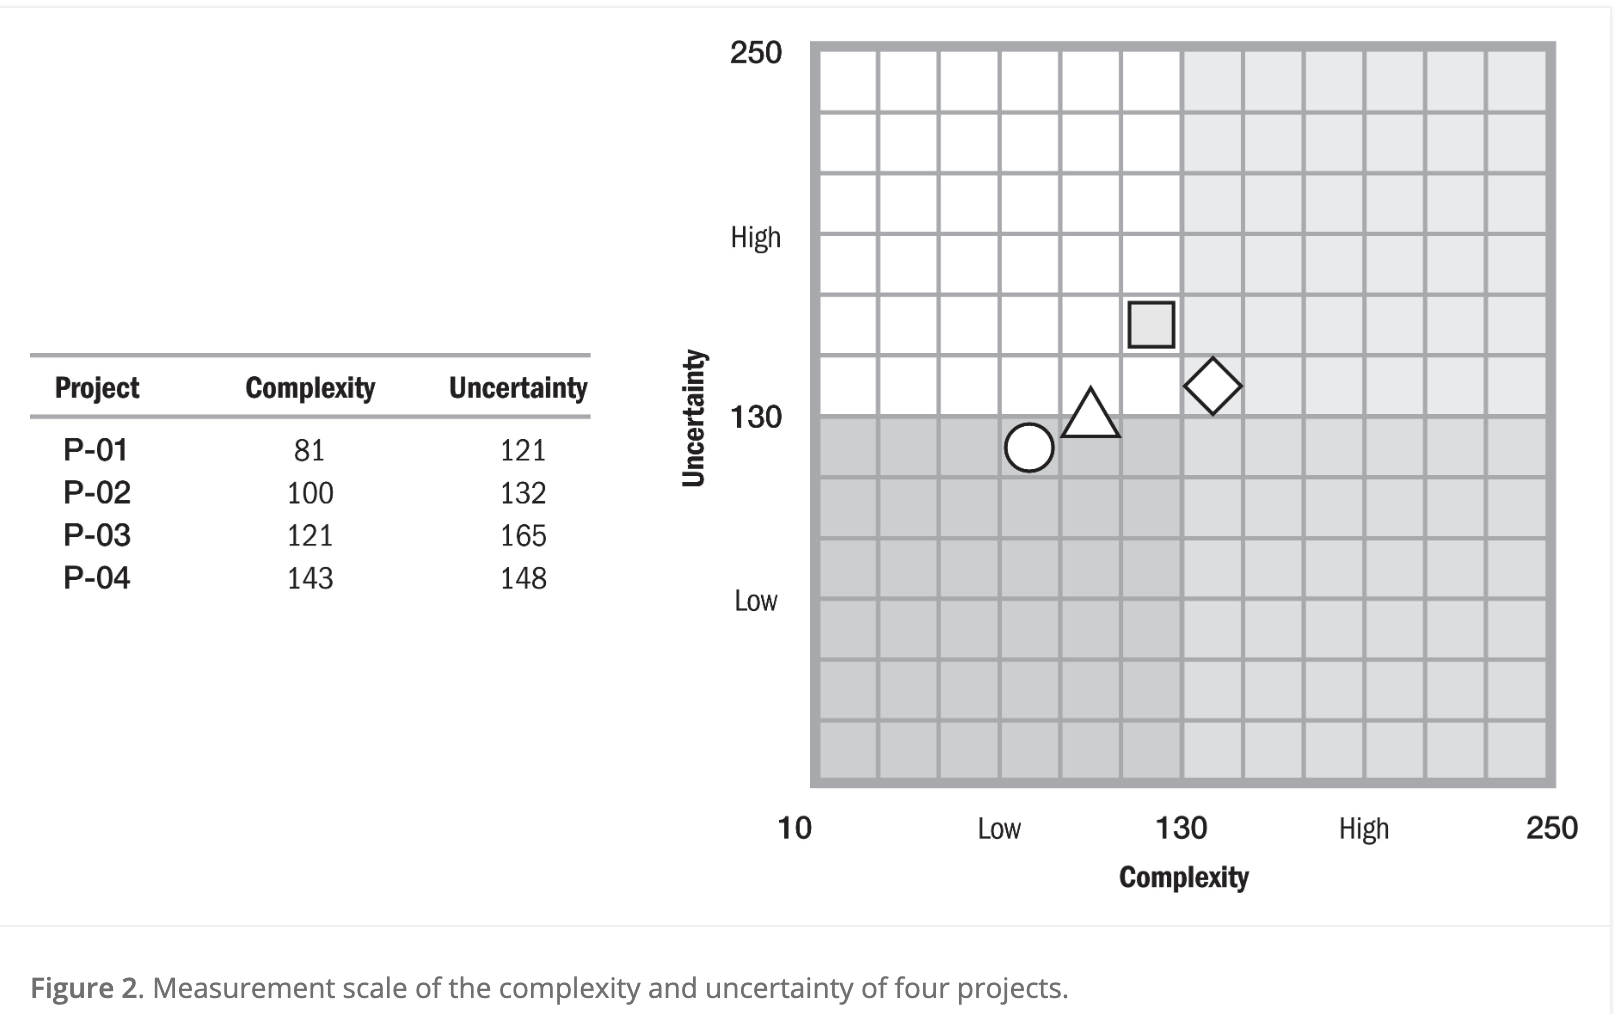
\includegraphics[width=0.8\linewidth]{Measurementscale.png}

                \end{figure}
    The case study examines a Brazilian mid-sized company (185 workers) in the construction tools sector. Selected for its complex, resource-intensive product development, high project uncertainty, and shared administration challenges, the study employs methods like defining variables, assessing complexity, using Critical Chain Project Management (CCPM) for planning, and validating results through logistic regression and expert judgment(coding interview).~\cite{refpaper7} \\
    The study employs a unique scale by Pinto et al. (2014) to assess project complexity and uncertainty simultaneously. Aligned with Vanhoucke's model, it maps projects on a Cartesian plane, highlighting CCPM suitability for high complexity and uncertainty. The questionnaire-based evaluation by eight project team members produces insightful classification points, guiding an understanding of project dynamics.~\cite{refpaper7}
                    \begin{figure}
                        \centering
                        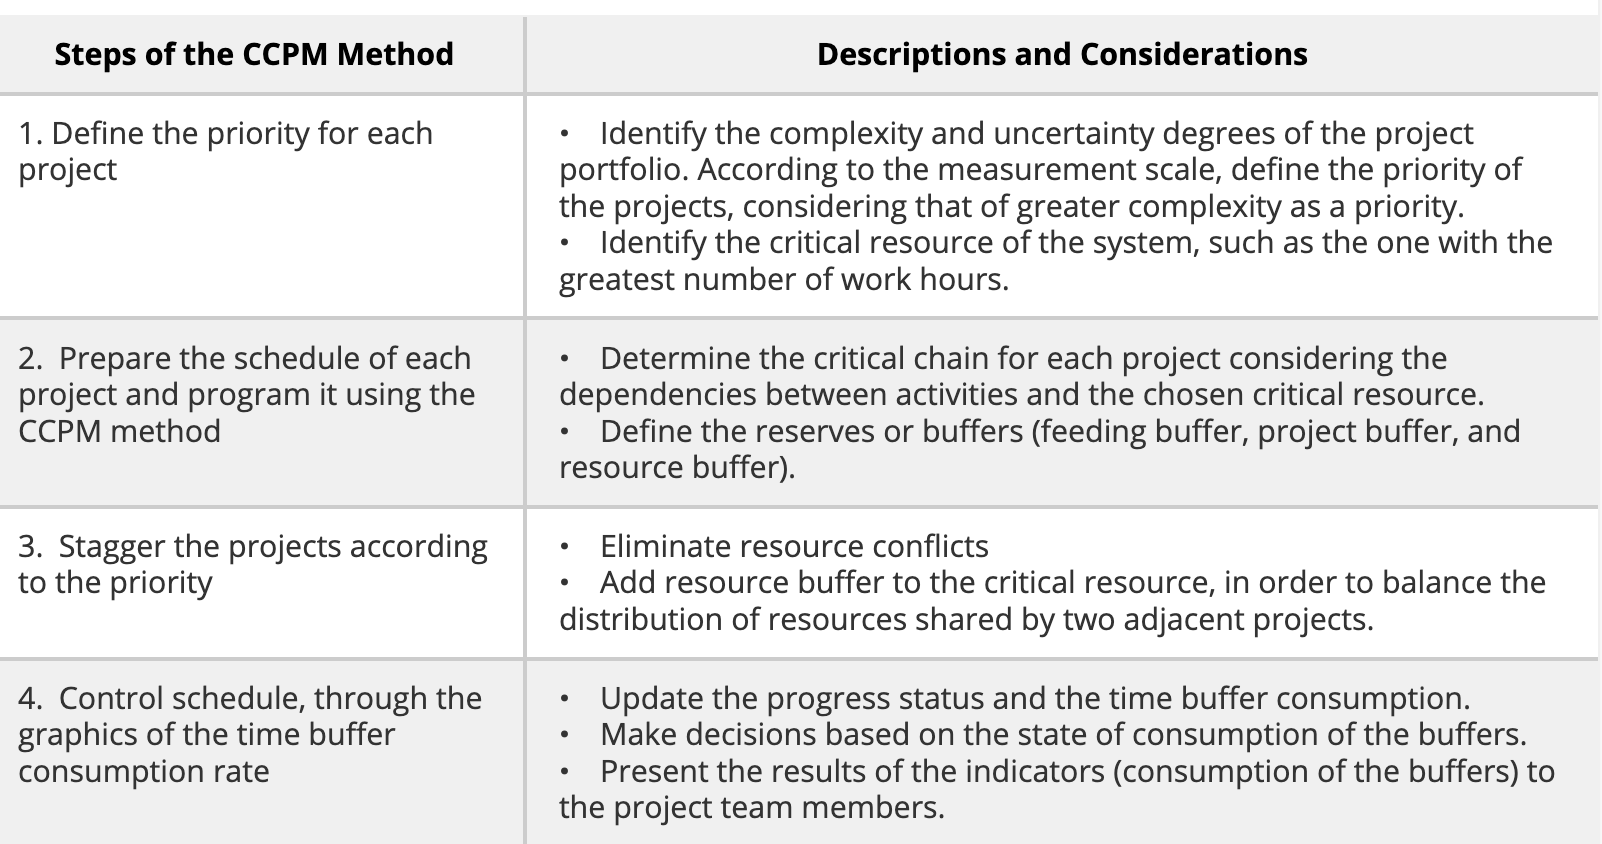
\includegraphics[width=0.85\linewidth]{StepsforCCPM.png}

                    \end{figure}
    The scale serves as a valuable tool to set a benchmark for resource prioritization, considering project complexity and uncertainty. Following this scale, the critical resource is sequenced from the least to the most complex projects: P-01, P-02, P-03, and P-04. This prioritization aligns with the projects' ascending order of complexity.~\cite{refpaper7} \\
    \textbf{Conclusion:}The findings and assessments suggest that constraining projects to the critical resource in a multiproject system, as advocated by the CCPM method, enhances workload distribution and simplifies activity monitoring and resource allocation as required and can also be implemented as a methodology for managing Multiple Interrelated projects and to decide the software tools needed.~\cite{refpaper7}
    \item\textbf{Project/Program Management Information System (PMIS):}
    Implement an effective PMIS for control and coordination.
    Ensure it allows for multi user check-out/check-in, coordinated updating, version maintenance, and alias naming.
    \item\textbf{Staffing Hierarchy Documentation:}
    Document the program’s staffing hierarchy clearly.
    Maintain an up-to-date roster with roles, responsibilities, project affiliations, and contact information.
    Include project leaders, program staff, and subject matter experts.
    \item \textbf{Delegated Responsibility:}
    Delegate responsibility to a program-level owner for managing the information in the PMIS. Ensure the program team has expertise in the technical tools and can provide support to contributors.
    Coordinate with software vendors to keep versions current and manage upgrades without disrupting the program.
    \item \textbf{Coordinating Program Plans:}
    Establish access to common computer scheduling tools for all projects.
    Provide planning templates and involve program staff in project startup workshops for consistency.Adopt computer-based project management software compatible with tools used by project leaders.
    \item \textbf{Online Time Tracking and Resource Monitoring:}
    Use server-based, centralized program tools for online time tracking and resource monitoring.
    Estimate time required to set up the database and include it in plans.
    \item \textbf{Standardized Status Collection and Reporting:}
    Standardize processes for status collection and reporting.
    Use compatible formats for data collection and coordinate project-level reporting for consistency.
    Set up the database for collecting status data online using high-end project management software.
    Provide access and training for program contributors.
\end{enumerate}




%----Tools to be used --- to use citation [2] here
\section{Results and Conclusion}
The observations drawn from the study above, emphasize the importance of meticulous planning and organization in managing large programs. It is recommended to assess and meet information requirements, especially those related to legal obligations and long-term storage by implementing various methods and methodologies in the industry.~\cite{refpaper8} Establishing a robust Project/Program Management Information System (PMIS) is highlighted as essential for effective control and coordination, with an emphasis on organizing online data for easy accessibility. ~\cite{refpaper8}~\cite{refpaper1}~\cite{refpaper2}The need for advanced software tools and methodologies like Kanban and Scrumban with features like multi user check-out/check-in, coordinated updating, and tailored security should be practiced. Clear documentation of the staffing hierarchy, delegating responsibility for managing information to a program-level owner etc should be the key points to always consider while deciding software tools for managing inter related multiple projects .~\cite{refpaper8} The coordination of program plans and monitoring progress is emphasized, suggesting the adoption of centralized project management tools for advantages in consistency.Standardizing processes for status collection and reporting is recommended, along with the use of compatible formats. \\
Overall, the observations stress the need for a comprehensive approach to information management, technology adoption, and coordination practices in large program settings.~\cite{refpaper8}~\cite{refpaper2}~\cite{refpaper10}
\subsection{Limitations}
To understnd the Limitations another case study was taken into consideration.~\cite{refpaper9}
\textbf{Case Study 2:} The case study focuses on the management of two interdependent software development projects within the company Entur during the COVID-19 pandemic. As technology companies shifted to remote work, the study explores how agile teams, particularly those in distributed settings, adapted to the challenges posed by the new work-from-anywhere (WFX) model. The central question addressed in the study is: "What coordination strategies are used by agile teams when working from anywhere?" To answer this question, empirical insights from an exploratory case study involving two developer teams, Team Alpha and Team Beta, are presented. Both teams are part of Entur, a public, mature, large-scale agile development company responsible for delivering digital infrastructure to the Norwegian public transport system.\\
\textbf{Research:} In detailing the case study, the research method involved a three-month investigation (November 2021 to January 2022) utilizing virtual interviews, observations of virtual stand-ups, and access to the virtual workspaces of the two teams. The study particularly emphasizes the period when national COVID-19 restrictions were lifted (24th September to 30th November 2021), allowing teams to choose their work locations. The findings reveal specific coordination strategies employed by the teams, addressing task selection, the use of communication tools (such as Discord, Slack, and Teams), and changes in meeting dynamics (unscheduled vs. scheduled). Notably, the teams had the autonomy to decide their work locations, and the study explores how this flexibility impacted their coordination strategies.~\cite{refpaper9}~\cite{refpaper10} \\
\textbf{Limitations Concluded:} Hence it can be concluded that,limitations an d challenges included the difficulties in scheduling unscheduled meetings in a virtual setting, the importance of physical co-location for certain types of tasks that require in-depth discussions, and the variations in communication tool effectiveness. The teams adopted tools like Discord to mimic co-located work practices, but challenges arose in virtual meeting scheduling, \textit{especially between interdependent teams} ~\cite{refpaper9}. Though there are new methodologies and methods being implimented still the challenges of interrelated project management remain and is an area that still needs further research.



\begin{thebibliography}{10}
\bibitem{refpaper1}
  M. C. J. Caniëls and R. J. J. M. Bakens, "The effects of Project Management Information Systems on decision making in a multi-project environment," \textit{International Journal of Project Management}, vol. 30, no. 2, pp. 162–175, Feb. 2012, doi: \url{https://doi.org/10.1016/j.ijproman.2011.05.005}.
\bibitem{refpaper2}
  S. Bathallath, Å. Smedberg, and H. Kjellin, "Managing project interdependencies in IT/IS project portfolios: a review of managerial issues," \textit{International Journal of Information Systems and Project Management}, vol. 4, no. 1, pp. 67–82, 2016, doi: \url{https://doi.org/10.12821/ijispm040104}.
‌\bibitem{refpaper3}
  R. Sweetman and K. Conboy, "Portfolios of Agile Projects," \textit{Project Management Journal}, vol. 49, no. 6, pp. 18–38, Oct. 2018, doi: \url{https://doi.org/10.1177/8756972818802712}.
\bibitem {refpaper4}
 M. Engwall and A. Jerbrant, "The resource allocation syndrome: the prime challenge of multi-project management?," \textit{International Journal of Project Management}, vol. 21, no. 6, pp. 403–409, Aug. 2003, doi: \url{https://doi.org/10.1016/s0263-7863(02)00113-8}.
\bibitem{refpaper5}
H. Bashir, U. Ojiako, A. Marshall, M. Chipulu, and A. A. Yousif,
\textit{The analysis of information flow interdependencies within projects},
\textit{Production Planning \& Control}, pp. 1–17, Sep. 2020,doi: \url{https://doi.org/10.1080/09537287.2020.1821115}.
\bibitem{refpaper6}
 M. Tanner and M. E. Dauane,\textit{The Use of Kanban to Alleviate Collaboration and Communication Challenges of Global Software Development},\textit{Issues in Informing Science and Information Technology},vol. 14,pp. 177–197,May 2017,
\url{https://www.informingscience.org/Publications/3716?Source=%2FJournals%2FIISIT%2FArticles%3FVolume%3D0-0}.
\bibitem{refpaper7}
R. E. C. Ordoñez, M. Vanhoucke, J. Coelho, R. Anholon, and O. Novaski,
``A Study of the Critical Chain Project Management Method Applied to a Multiproject System,''\emph{Project Management Journal}, vol. 50, no. 3, pp. 322–334, Mar. 2019,doi: \url{https://doi.org/10.1177/8756972819832203}.
\bibitem{refpaper8}
S. Y. Chadli, A. Idri, J. N. Ros, J. L. Fernández-Alemán, J. M. C. de Gea, and A. Toval, \\ \emph{Software project management tools in global software development: a systematic mapping study}, \emph{SpringerPlus}, vol. 5, no. 1, Nov. 2016,doi: \url{https://doi.org/10.1186/s40064-016-3670-7}.
\bibitem{refpaper9}
T. Sporsem and N. B. Moe, \emph{Coordination Strategies When Working from Anywhere: A Case Study of Two Agile Teams},\emph{Lecture Notes in Business Information Processing}, vol. 5, no. 1, Nov. 2022, \\
doi: \url{https://doi.org/10.1007/978-3-031-08169-9_4}.
\bibitem{refpaper10}
V. Stray and N. B. Moe,\emph{Understanding coordination in global software engineering: A mixed-methods study on the use of meetings and Slack},\emph{Journal of Systems and Software}, vol. 170, p. 110717, Dec. 2020,doi: \url{https://doi.org/10.1016/j.jss.2020.110717}.‌
‌
‌
\end{thebibliography}



\section{Acknowledgements}
I am grateful to ChatGPT, Perplexity, and a few YouTube channels for their important help and insights, which made this effort much better. Furthermore, references from academic journals that can be accessed via Google Scholar have been included.




\end{document}